
\chapter{The Zeta Function of Riemann (Contd).}\label{chap16}

\medskip
\noindent{\textbf{Hamburger's Theorem.}}\cite{key13}\pageoriginale

We have seen that the functional equation of the Gamma function,
together with its logarithmic convexity, determine the Gamma function
`essentially' uniquely (i.e. up to a constant). A corresponding
result can be proved for a the zeta function.

\setcounter{thm}{0}
\begin{thm}\label{chap16:thm1}
Let $f(s) = \dfrac{G(s)}{P(s)}$, where $G(s)$ is an entire function of
finite order and $P(s)$ is a polynomial, and let
\begin{equation*}
f(s) = \sum\limits^\infty_{n=1} \frac{a_n}{n^s}, \tag{1.1}\label{c16:eq1.1}
\end{equation*}
the series on the right converging absolutely for $\sigma >1$.

Let 
\begin{equation*}
f(s) \Gamma \left(\frac{s}{2} \right) \pi^{-s/2} = g(1-s)
\Gamma \left(\frac{1}{2} -\frac{s}{2} \right) \pi^{-\frac{(1-s)}{2}} \tag{1.2}\label{c16:eq1.2}
 \end{equation*}
where 
\begin{equation*}
g(1-s) = \sum\limits^\infty_{n=1} \frac{b_n}{n^{1-s}}, \tag{1.3}\label{c16:eq1.3}
\end{equation*} 
The series on the right converging absolutely for $\sigma < - \alpha <
0$. Then $f(s) = a_1 \zeta(s) (=g(s))$.
\end{thm}

For the proof we need to evaluate two integrals:
\begin{gather*}
e^{-y} = \frac{1}{2\pi i} \int\limits^{1+\infty i}_{1-\infty i} y^{-s}
\Gamma(s) ds, \quad y > 0\tag{1}\label{c16:eq1}\\
\int\limits^{\infty}_0 e^{-a^2x -\frac{b^2}{x}}  \frac{dx}{\surd x} =
\frac{\surd \pi}{a} e^{-2ab}, \quad a>0, \quad b \geq 0. \tag{2}\label{c16:eq2}
\end{gather*}\pageoriginale

The first formula is a classic example of \textit{Mellin's inversion
  formula} which can be obtained as an instance of Fourier's inversion
formula discussed in the last lecture. We have seen that if $f(x)
\in L_1 (-\infty, \infty)$, then its Fourier transform $\phi(\alpha)$
is defined in $-\infty < \alpha < \infty$, and if in a neighbourhood
of $x_0$, $f(x)$ is differentiable, then
$$
f(x_0) = \frac{1}{2\pi} \int\limits^\infty_{-\infty} e^{-ix_0\alpha} d
\alpha \int\limits^\infty_{-\infty} f(y) e^{i\alpha y} dy.
$$

If we define
\begin{equation*}
 \mathscr{F} (s) = \int\limits^\infty_0 f(x) x^{s-1} dx, \tag{3}\label{c16:eq3}
\end{equation*}
for $s = c+ it$, $c>0$, where $f(x) x^{c-1}\in L_1 (0,\infty)$, so
that the integral on the right exists absolutely, we can look upon
this as a Fourier transform by a change of variable: $x\to e^y$, for 
$$
\mathscr{F} (c+it) = \int\limits^\infty_{-\infty} f(e^y) e^{yc} e^{it
  \; y}  dy
$$
Hence, provided that $f(e^y) e^{yc}$ satisfies a suitable `local'
condition, such as differentiability in the neighbourhood of a point,
we can invert this relation and obtain
$$
f(e^y) \cdot e^{yc} = \frac{1}{2\pi} \int\limits^\infty_{-\infty}
\mathscr{F} (c+it) e^{-iyt} dt
$$
or\pageoriginale
\begin{align*}
f(e^y) & = \frac{1}{2\pi} \int\limits^\infty_{-\infty} \mathscr{F}
(c+it) e^{-(c+it)y} dt\\
& = \frac{1}{2\pi i} \int\limits^{c+i\infty}_{c-i\infty} \mathscr{F}
(s)  e^{-ys} ds\\
\text{or } \qquad f(x) & = \frac{1}{2\pi i}
\int\limits^{c+i\infty}_{c-i\infty} \mathscr{F}(s) x^{-s} ds, \; c>0. \tag{4}\label{c16:eq4}
\end{align*}

Relations (\ref{c16:eq3}) and (\ref{c16:eq4}) give the Mellin inversion formulae. 
Since $\Gamma(s) = \int\limits^\infty_0 e^{-x} x^{s-1} dx$, $\re s
>0$, we get (\ref{c16:eq1}) as in immediate application.

We know that, for $k>0$
$$
\int\limits^A_0 e^{-(k-i\alpha)x} dx = \frac{1}{k-i\alpha}
\left(1-e^{-kA} e^{i\alpha A} \right)
$$
so that
$$
2 \int\limits^\infty_0 e^{-kx} \cos \alpha x dx = \frac{2.k}{k^2+\alpha^2}
$$
and by Fourier's inversion formula,
\begin{equation*}
\int\limits^\infty_0 \frac{\cos \alpha x}{k^2 + \alpha^2} d \alpha =
\frac{\pi e^{-kx}}{2k}, \quad k>0 \tag{5}\label{c16:eq5}
\end{equation*}
On the other hand, we have for $k \geq 0$
$$
\frac{\Gamma(1)}{x^2 + k^2} = \int\limits^\infty_0 e^{-(x^2 + k^2)y} dy,
$$
so that\pageoriginale
\begin{align*}
\int\limits^\infty_0 \frac{\cos \alpha x}{x^2+k^2} dx & = \frac{\surd
  \pi}{2} \int\limits^\infty_0 y^{-\frac{1}{2}} e^{-(k^2 y +
  \frac{\alpha^2}{4y})} dy\\
& = \frac{\pi}{2k} e^{-|\alpha|k} , \text{ from (\ref{c16:eq5})}.
\end{align*}
Setting $k^2 = a^2$, $\alpha^2 = 4b^2$, we get
$$
\int\limits^\infty_0 e^{-a^2 x -\frac{b^2}{x}} \frac{dx}{\surd x} =
\frac{\surd \pi }{a} e^{-2ab}, a > 0 \;  b\ge 0
$$
which proves formula (\ref{c16:eq2}).

\medskip
\noindent{\textbf{Proof of Theorem 1.}}
For any $x>0$, we have by (\ref{c16:eq1.1}) and (\ref{c16:eq1.2}), (Here $f(s)=O(1)$)
\begin{align*}
S_1 & \equiv \frac{1}{2\pi i} \int\limits^{2+i\infty}_{2-i\infty} f(s)
\Gamma \; \frac{(s)}{2} \;  \pi^{(-s/2)} \cdot x^{-s/2} ds\\
& = \sum\limits^\infty_{n=1} \frac{a_n}{2\pi i}
\int\limits^{2+i\infty}_{2-i\infty} \Gamma(s/2) (\pi n^2 x)^{-s/2}
ds\\
& = 2 \sum\limits^\infty_{n=1} a_n e^{-\pi n^2x}
\end{align*}

We have, however, by (\ref{c16:eq1.2}), $S_1 = S_2$, where 
$$
S_2 = \frac{1}{2\pi i} \int\limits^{2+i\infty}_{2-i\infty} g(1-s) 
\Gamma \left(\frac{1-s}{2} \right)  \pi^{\frac{-(1-s)}{2}} x^{-s/2} ds.
$$\pageoriginale
Now we wish to move the line of integration here from $\sigma =2$ to
$\sigma = -1-\alpha$.

By the hypothesis on the `order' of $f(s)$ and (\ref{c16:eq1.2}), it follows that
there exist two numbers $T>0$, $\gamma>0$, such that for $|t| \geq T$
and $-1 - \alpha \leq \sigma \leq 2$, the function $g(1-s)$ is regular
and $O(e^{|t|^\gamma})$. By (\ref{c16:eq1.3}), we see that $g(1-s) = O (1)$ on
$\sigma =-1 - \alpha$; and, since $f(s) = O(1)$ on $\sigma =2$, while 
$$
\frac{\Gamma(s/2)}{\Gamma(\frac{1-s}{2})} = O (|t|^{3/2}), \text{ on }
\sigma =2, 
$$
it follows that $g(1-s) = O (|t|^{3/2})$ on $\sigma =2$. Hence, by the
principle of Phragmen-Lindel\"of, we observe that
$$
g(1-s) = O (|t|^{3/2})
$$
for $|t| \geq T$, $-\alpha -1 \leq \sigma \leq 2$. \textit{Taking a
  suitable rectangle, and applying Cauchy's theorem}, we get
$$
S_2 = \frac{1}{2\pi i} \int\limits^{-\alpha -1+i\infty}_{-\alpha -1-i
  \infty} g(1-s) \Gamma\left(\frac{1-s}{2} \right)
\pi^{-\frac{(1-s)}{2}} x^{-s/2} ds + \sum\limits^{m}_{v=1} R_\nu
$$
\begin{figure}[H]
\centering
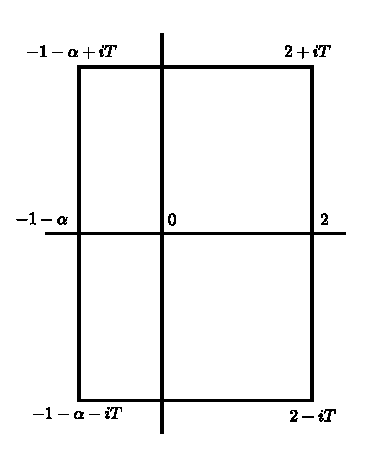
\includegraphics{figures/fig16.1.eps}
\end{figure}

\noindent
where $R_\nu$ is the residue of the integrand at the pole $s_\nu$
lying in the region\pageoriginale $-\alpha -1 < \sigma < 2$. The
integrand, however, equals
$$
f(s) \Gamma\left(\frac{s}{2} \right) \pi^{-s/2} x^{-s/2} 
$$
The residue of this at a pole $s_\nu$ of order $q_{\nu}$ is 
$$ 
x^{\frac{-s_\nu}{2}} \left(A^{(\nu)}_{q_\nu-1} \log^{q_\nu-1} x + \cdots +
A^{(\nu)}_1 \log x + A^{(\nu)}_0\right)
$$
Hence
\begin{align*}
\sum^m_{\nu=1} R_\nu = \sum^m_{\nu=1} x^{-s_\nu/2} & Q_\nu (\log x) =
Q(x), \text{ say, where}\\
& \quad Q_\nu \text{ is a polynomial}
\end{align*}
Here $\re s_\nu \leq 2 - \theta$, $\theta >0$. (i.e. we are using the
absolute convergence of $\sum a_n n^{-s}$ only for $\sigma > 2 - \theta$).

Hence
\begin{align*}
S_2 & = \frac{1}{\surd x} \sum\limits^\infty_{n=1} \frac{b_n}{2\pi i}
\int\limits^{-\alpha - 1 + i \infty}_{-\alpha - 1 - i \infty} \frac{\Gamma(1-s)}{2} \left(\frac{\pi n^2}{x} \right)^{-\frac{(1-s)}{2}} ds
+ Q (x)\\
& = \frac{2}{\surd x} \sum\limits^\infty_{n=1} \frac{b_n}{2\pi i}
\int\limits^{\frac{\alpha}{2} + 1 + i \infty}_{\frac{\alpha}{2} + 1 -
  i \infty}  \Gamma(s) \left(\frac{\pi n^2}{x} \right)^{-s} ds +
Q(x)\\
& = \frac{2}{\surd x} \sum\limits^{\infty}_{n=1} b_n e^{-\pi n^2/x} +
Q(x) 
\end{align*}

Hence\pageoriginale (since $S_1 = S_2$) we have 
$$
2 \sum\limits^\infty_1 a_n e^{-\pi n^2 x} = \frac{2}{\surd x}
\sum\limits^\infty_{n=1} b_n e^{-\pi n^2/x} + Q(x)
$$
Multiplying this by $e^{-\pi t^2 x}$, $t>0$, and integrating over
$(0,\infty)$ w.r.t. $x$, we get
$$
2 \sum\limits^\infty_{n=1} \frac{a_n}{\pi(t^2+n^2)} = 2 
\sum\limits^\infty_{n=1} \frac{b_n}{t} e^{-2\pi nt} +
\int\limits^\infty_0 Q (x) e^{-\pi t^2 x }dx
$$
by (\ref{c16:eq2}).

The last integral is convergent. Since $\re s_\nu \leq 2 - \theta$,
$\nu=1,2,\ldots m$, each term of $Q(x)$ is
$O(x^{-1+\frac{\theta}{4}})$ as $x\to 0$.

Now
$$
\int\limits^\infty_0 Q (x)e^{-\pi t^2x} dx = \frac{1}{t^2}
\int\limits^\infty_0 Q \left(\frac{x}{t^2} \right) e^{-\pi x} dx =
\sum\limits^m_1 t^{s_\nu -2}  H_\nu (\log t),
$$
where $H_\nu$ is a polynomial, $= H(t)$, say.
 
Hence
$$
\sum\limits^\infty_{n=1} a_n \left( \frac{1}{t+ni} +
\frac{1}{t-ni}\right) - \pi t H(t) = 2 \pi \sum\limits^\infty_{n=1}
b_n e^{-2\pi nt}
$$
The series on the left hand side is uniformly convergent in any finite
region of the $t$-plane which excludes $t=\pm ki$, $k=1,2,\ldots;$ It
is a meromorphic function with poles of the first order at $t=\pm ki$.

$H(t)$\pageoriginale is regular and single-valued in the $t$-plane
with the negative real axis deleted and $t \neq 0$.

The right hand side is a periodic function of $t$ with period $i$ for
$\re t >0$. Hence, by analytical continuation, so is the function on
the left. Hence the residues at $ki$, $(k+1)i$ are equal. So $a_k =
a_{k+1}$


